Há três tipos de ambientes no desenvolvimento desta aplicação: \textit{development}, \textit{staging} e \textit{production}. O ambiente de \textit{development}, ou desenvolvimento, é o ambiente local de cada desenvolvedo; \textit{staging} ou pré-produção é um ambiente para serem realizados testes beta e \textit{production}, ou produção, é o ambiente final onde a aplicação será de fato utilizada pelos usuários.

Na API, a integração contínua é feita com a ferramenta TravisCI, onde, quando um \textit{pull request} é aceito na \textit{branch staging}, o Travis executa toda a suíte de testes para identificar se algum deles pode ter resultado em falha. Caso todos passem, ele verifica se todas as métricas definidas pelo Rubocop estão de acordo com o padrão definido. Caso todas as métricas passem, a \textit{build} de pré produção é criada, o Travis envia as informações de cobertura de testes para o Coveralls, as informações de métricas para o Code Climate e em seguida realiza o \textit{deploy} no ambiente de pré produção no Heroku.

Se um \textit{pull request} for aceito na \textit{branch} \textit{master} todo o processo será o mesmo, exceto pelo \textit{deploy}, que ocorrerá no ambiente de produção no Heroku.

A Figura \ref{img:integracao_deploy_continuo_api} ilustra o processo de integração e \textit{deploy} contínuo feito na API.

\begin{figure}[H]
    \centering
    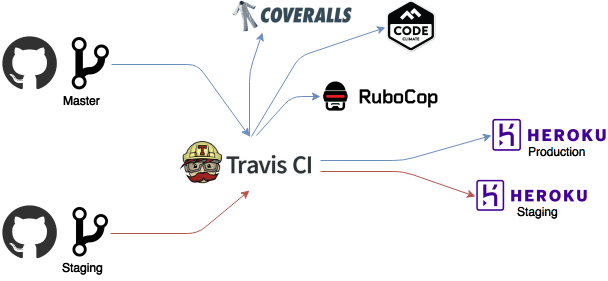
\includegraphics[scale=0.5]{figuras/api_ci.png}
    \caption[Integração e \textit{deploy} contínuo na API]{Integração e \textit{deploy} contínuo API. Fonte: autores}
    \label{img:integracao_deploy_continuo_api}
\end{figure}
\pagebreak
No aplicativo planejou-se a integração e o \textit{deploy} contínuo como mostra a Figura \ref{img:integracao_deploy_continuo_planejado_app}.

\begin{figure}[H]
    \centering
    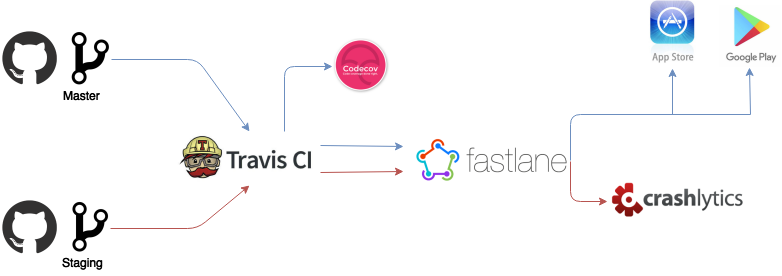
\includegraphics[scale=0.5]{figuras/ci_should_be.png}
    \caption[Integração e \textit{deploy} contínuo planejado para o aplicativo]{Integração e \textit{deploy} contínuo planejado para o aplicativo. Fonte: autores}
    \label{img:integracao_deploy_continuo_planejado_app}
\end{figure}

Se um \textit{pull request} for aceito na \textit{branch master}, o Travis realizará toda a suíte de testes; caso todos passem, ele enviará as informações de cobertura para o Codecov e através do Fastlane realizará o \textit{deploy} do aplicativo, tanto na Play Store quanto na App Store. Se um \textit{pull request} for aceito na \textit{branch staging}, todo o processo será repetido, exceto pelo fato que o deploy do aplicativo não é realizado nas lojas e sim no Crashlytics, que irá criar a versão beta do aplicativo e o enviará para os e-mails previamente configurados.

Para a primeira entrega do trabalho, foi planejado só até o \textit{deploy} beta, como mostrado na Figura \ref{img:integracao_deploy_continuo_planejado_primeira_entrega}:

\begin{figure}[H]
    \centering
    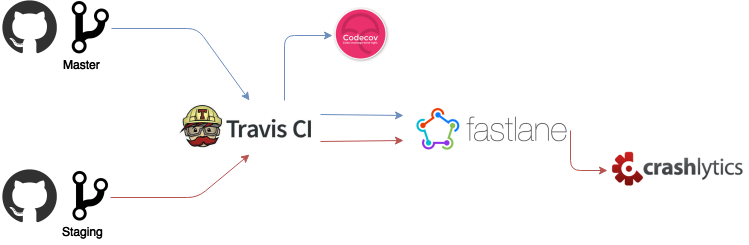
\includegraphics[scale=0.5]{figuras/ci_as_is.png}
    \caption[Integração e \textit{deploy} contínuo planejado para a primeira entrega]{Integração e \textit{deploy} contínuo planejado para a primeira entrega. Fonte: autores}
    \label{img:integracao_deploy_continuo_planejado_primeira_entrega}
\end{figure}

Entretanto, não foi possível fazer com que o \textit{deploy} contínuo acontecesse logo após a integração contínua, um desafio causado pela escolha de desenvolvimento híbridos de aplicativo. Uma vez que o código versionado do aplicativo é o mesmo código para a plataforma Android e iOS, e após realizar a \textit{build} desse código são gerados códigos em cada plataforma, não versionados. A ferramenta de integração contínua não consegue ter acesso aos códigos de cada plataforma para realizar os devidos \textit{deploys}. Sendo assim, o \textit{deploy} contínuo estava acontecendo manualmente através do comando:

\begin{lstlisting}[language=bash]
  $ fastlane beta
\end{lstlisting}

A Figura \ref{img:integracao_deploy_continuo_atual} ilustra como estava funcionando a integração e o \textit{deploy} contínuo do aplicativo até a primeira entrega.

\begin{figure}[H]
    \centering
    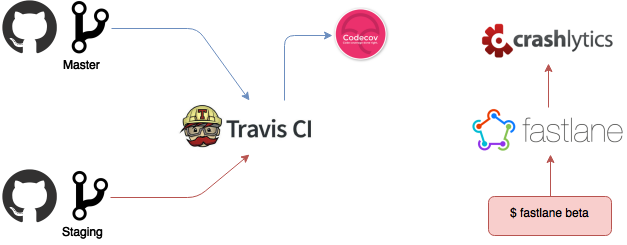
\includegraphics[scale=0.5]{figuras/ci_currently.png}
    \caption[Integração e \textit{deploy} contínuo atual]{Integração e \textit{deploy} contínuo até a primeira entrega. Fonte: autores}
    \label{img:integracao_deploy_continuo_atual}
\end{figure}

Na segunda parte do trabalho foram avaliadas formas de melhorar essa automatização. Entretanto, com o lançamento da versão 3 do Ionic, muitas dependências pararam de funcionar e a automatização, que deveria economizar tempo, rodando os testes e integrando as novas funcionalidades ao aplicativo e realizando o \textit{deploy} nas lojas, começou a ocasionar perda de tempo de desenvolvimento na tentativa de integrar ferramentas para as quais o Ionic não oferece suporte. Portanto, decidiu-se remover a integração e entrega contínua do aplicativo e realizar essas tarefas manualmente, deixando assim essa melhoria como proposta para trabalhos futuros.
